\documentclass{bmvc2k}
\usepackage[parfill]{parskip}


%% Enter your paper number here for the review copy
% \bmvcreviewcopy{??}

\title{Pr�ctica 1: Clasificadores generativos}

% Enter the paper's authors in order
% \addauthor{Name}{email/homepage}{INSTITUTION_CODE}
\addauthor{Jorge S�ez Tejedor}{j.saez.2016@alumnos.urjc.es}{1}

% Enter the institutions
% \addinstitution{Name\\Address}
\addinstitution{
 M�ster Oficial de Visi�n Artificial\\
 Universidad Rey Juan Carlos\\
 Campus de Mostoles, Espa�a
}

\renewcommand*\contentsname{Contenidos}
\renewcommand*\figurename{Figura}

\runninghead{}{}

% Any macro definitions you would like to include
% These are not defined in the style file, because they don't begin
% with \bmva, so they might conflict with the user's own macros.
% The \bmvaOneDot macro adds a full stop unless there is one in the
% text already.
\def\eg{\emph{e.g}\bmvaOneDot}
\def\Eg{\emph{E.g}\bmvaOneDot}
\def\etal{\emph{et al}\bmvaOneDot}

%-------------------------------------------------------------------------
% Document starts here
\begin{document}

\maketitle

El objetivo de esta practica es conocer y emplear la biblioteca Sk-Learn para entrenar y testear varios clasificadores con diferentes conjuntos de datos.

Para ello se dispone de un script en Python que genera los datos de test y entrenamiento, a continuaci�n se presentan esos datos a diferentes clasificadores que realizan una b�squeda de par�metros �ptimos mediante \textit{cross validation} 5-Fold. Una vez encontrados se entrena un clasificador con esos par�metros y se eval�a su rendimiento.

En este documento se muestran los resultados, en primer lugar, cada uno de los datos de entrenamiento y test representados gr�ficamente, a continuaci�n la salida de texto del script Python y por ultimo el resultado de cada uno de los clasificadores entrenados con los par�metros �ptimos. 

\section{Resultados con Gaussianas 1}

\begin{figure}[!ht]
	\centering
	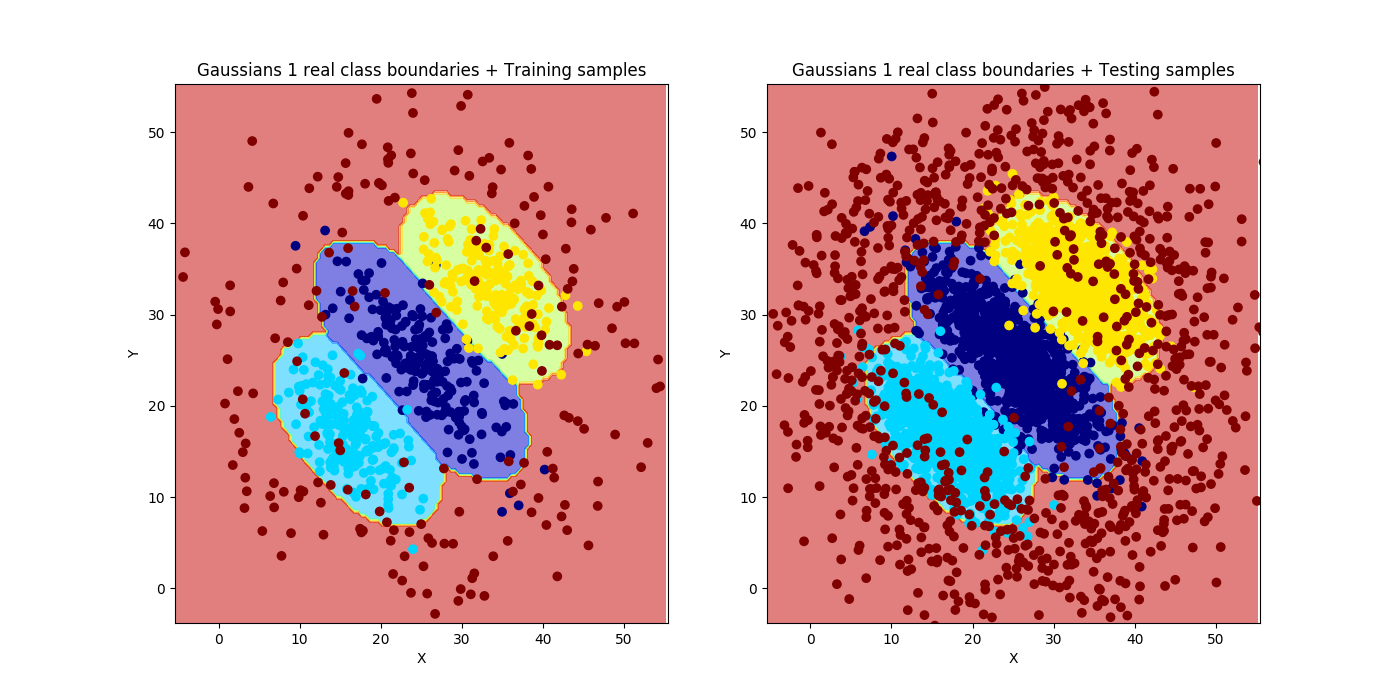
\includegraphics[width=0.8\linewidth]{figs/1-aTest}
	\caption{Conjunto de muestra 1}
	\label{fig:1-atest}
\end{figure}

El resultado obtenido para el conjunto de Gaussianas numero 1 es el siguiente:

\texttt{\small{Gaussian Bayes (Test) Done. Score: 0.92 \\
	GMM Sk-Learn Done. Score: 0.92  n = [2, 2, 3, 2] \\ Cov = ['diag', 'tied', 'diag', 'tied']\\
	KNN Done. Score: 0.91  K = 6 Weights = distance\\
	Parzen Done. Score: 0.78  r = 25 Weights = distance}}


\begin{figure}[!ht]
	\centering
	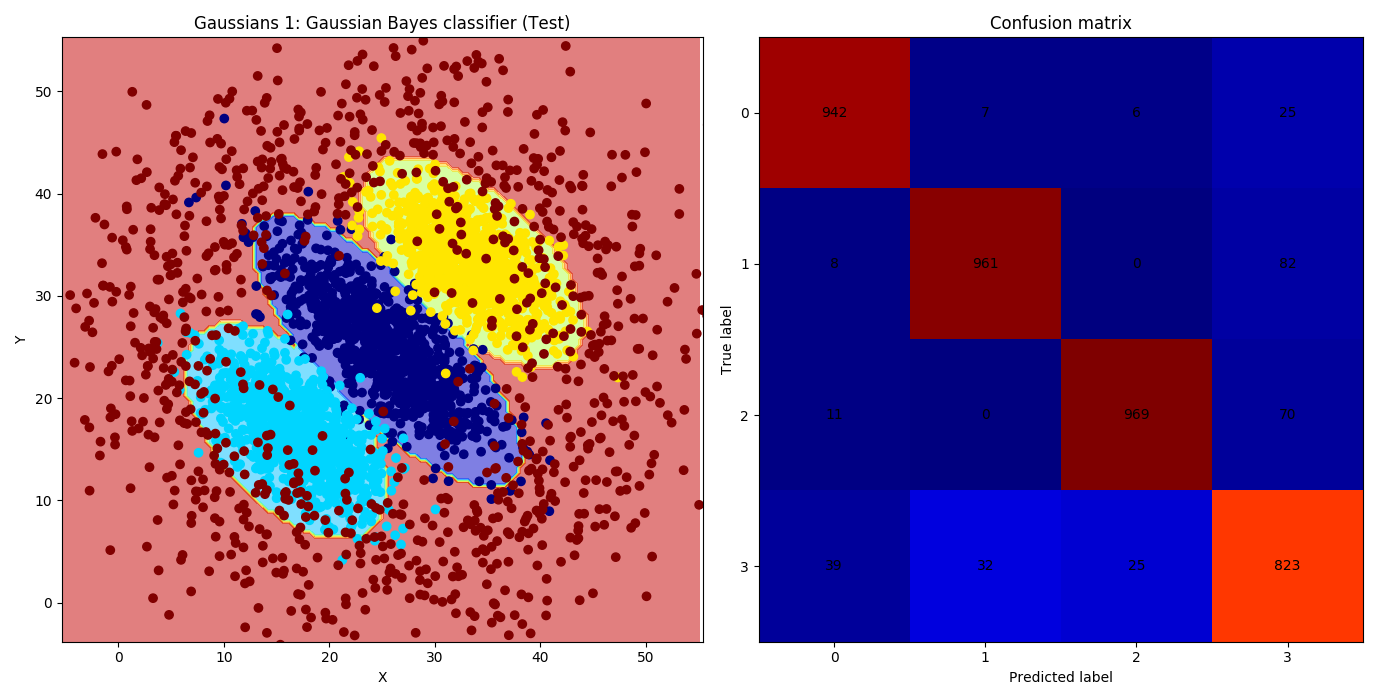
\includegraphics[width=0.8\linewidth]{figs/1-Bayes}
	\caption{Resultado del conjunto 1 con clasificador de Test Bayesiano}
	\label{fig:1-Bayes}
\end{figure}

\begin{figure}[!ht]
	\centering
	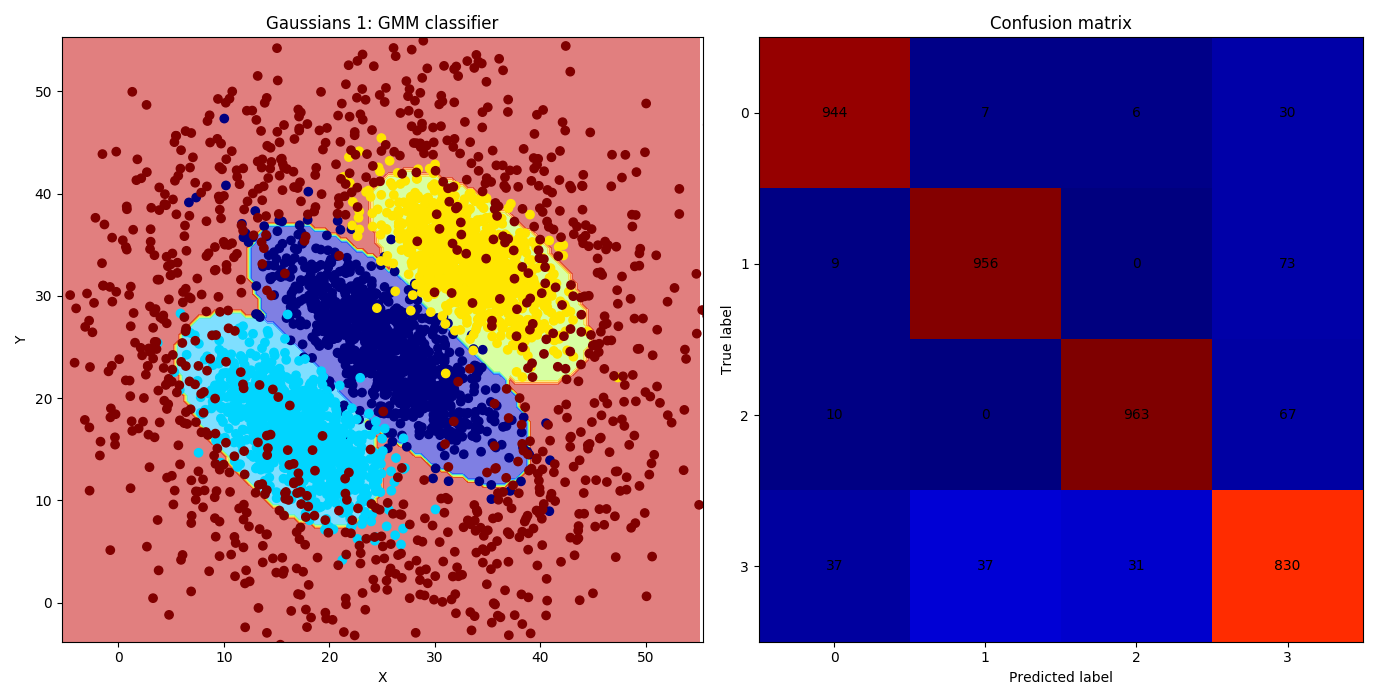
\includegraphics[width=0.8\linewidth]{figs/1-GMM}
	\caption{Resultado del conjunto 1 con clasificador de mezcla de gaussianas}
	\label{fig:1-GMM}
\end{figure}

\begin{figure}[!ht]
	\centering
	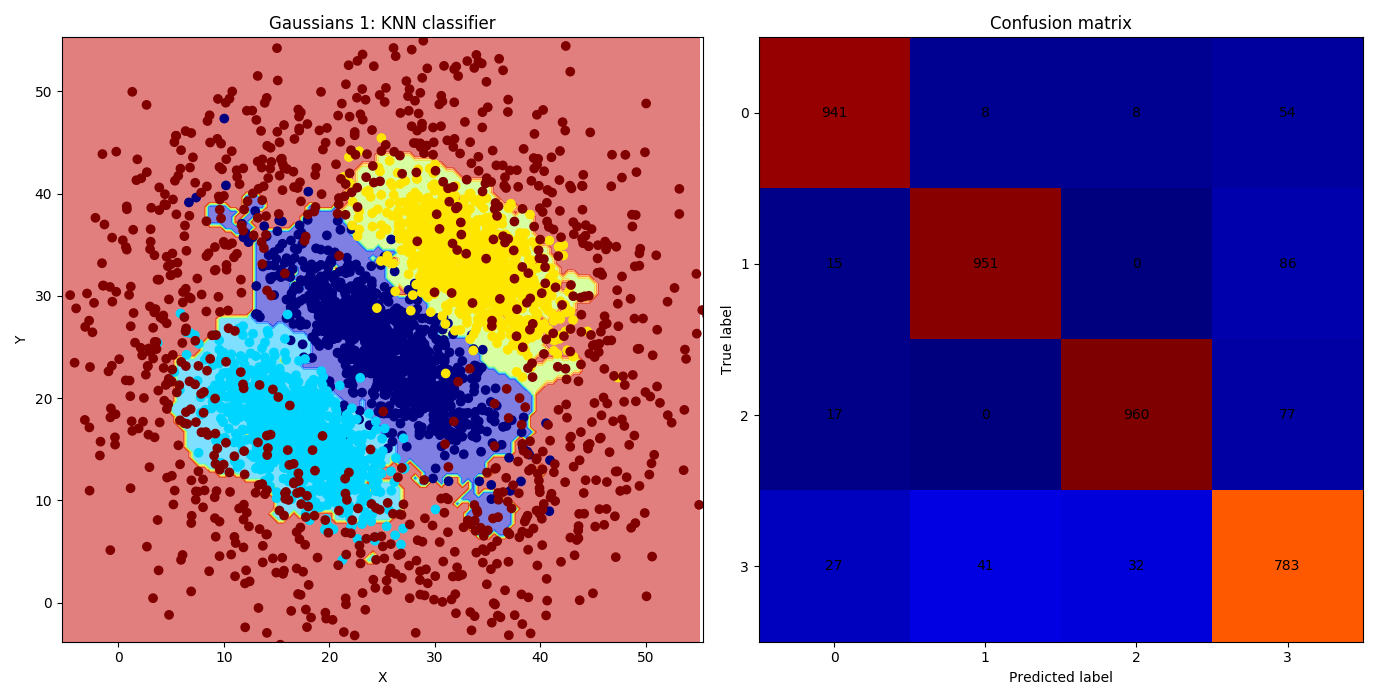
\includegraphics[width=0.8\linewidth]{figs/1-KNN}
	\caption{Resultado del conjunto 1 con clasificador de Vecinos mas cercanos (KNN)}
	\label{fig:1-KNN}
\end{figure}

\begin{figure}[!ht]
	\centering
	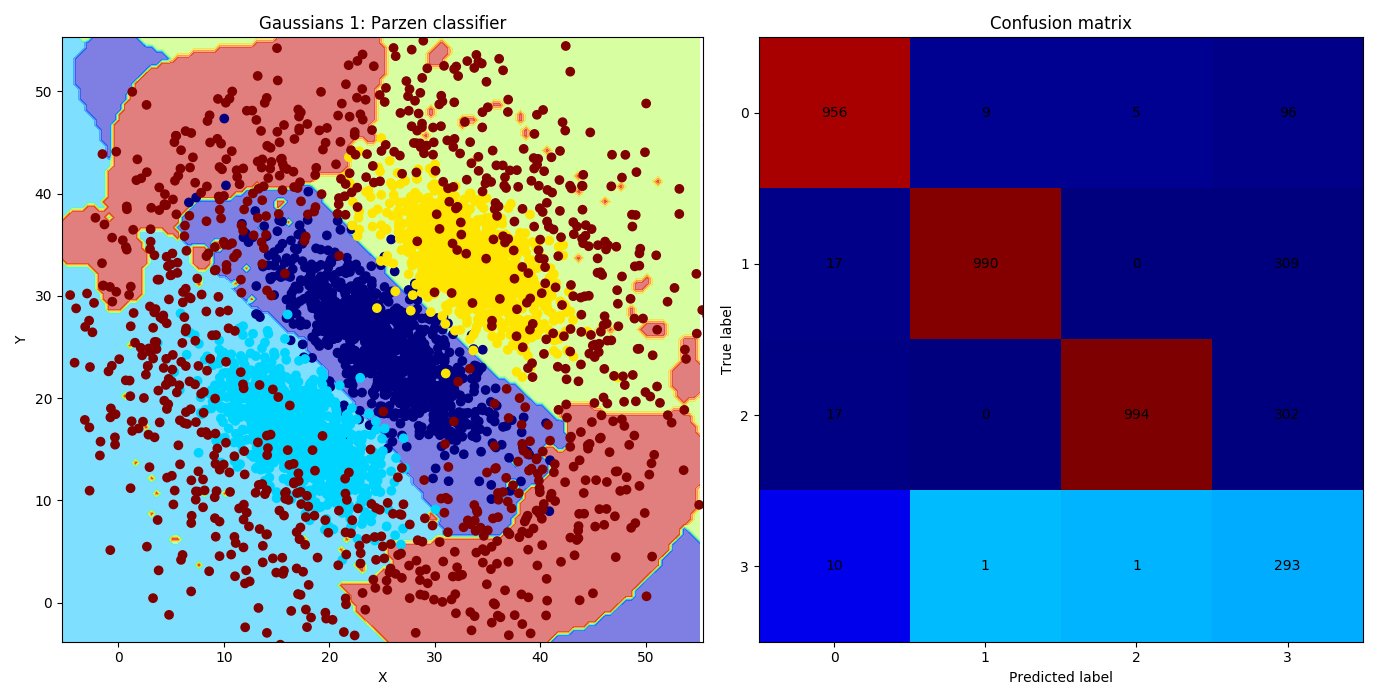
\includegraphics[width=0.8\linewidth]{figs/1-Parzen}
	\caption{Resultado del conjunto 1 con clasificador basado en ventanas de Parzen}
	\label{fig:1-Parzen}
\end{figure}

A la vista de los resultados, el mejor clasificador para este conjunto de entrenamiento se trata del basado en mezcla de gaussianas, es un resultado mas que esperado ya que, como se puede ver en la Figura \ref{fig:1-atest}, 3 de las 4 clases tienen una gran semejanza a gaussianas con matriz de covarianza diagonal, de hecho el clasificador elije este tipo en 2 de las 4. 

Como se puede ver en la Figura \ref{fig:1-Parzen} el clasificador basado en ventanas de Parzen tiene grandes dificultades a la hora de adecuarse a la forma que presentan los datos, sobre todo en las fronteras de la clase 3.

\clearpage
\section{Resultados con Gaussianas 2}

\begin{figure}[!ht]
	\centering
	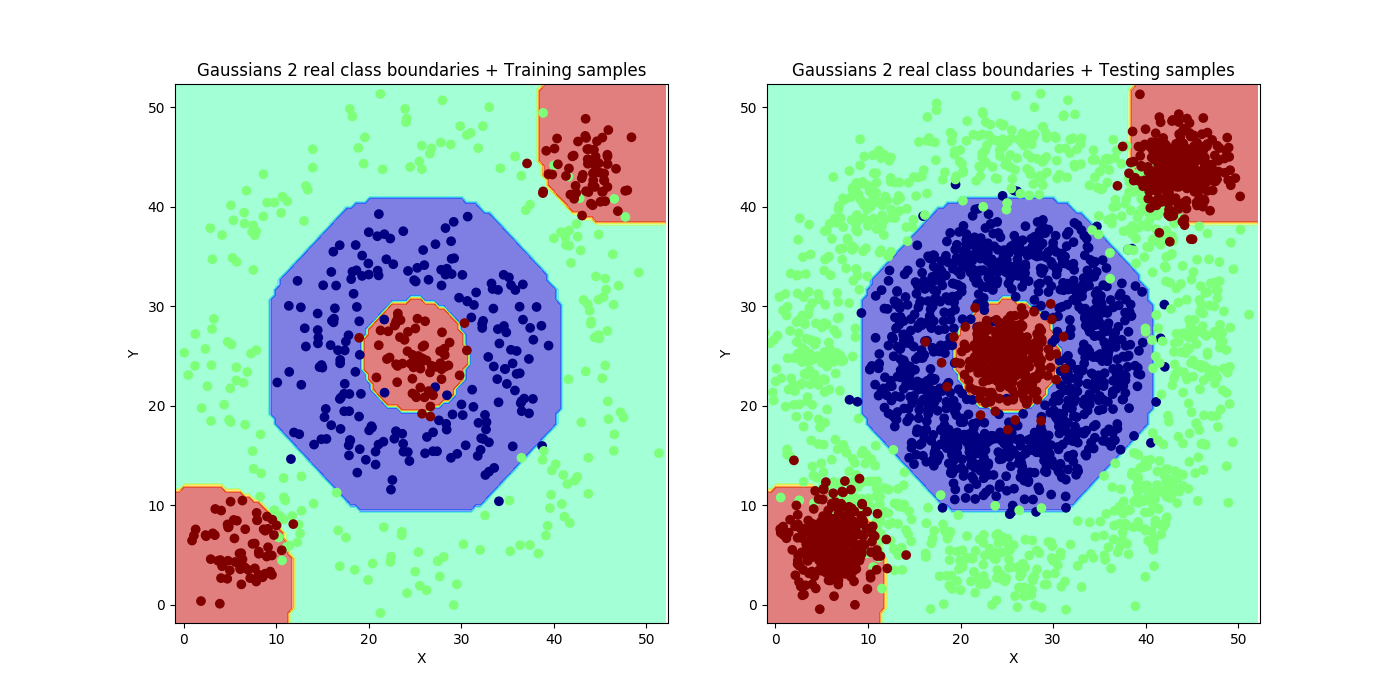
\includegraphics[width=0.8\linewidth]{figs/2-aTest}
	\caption{Conjunto de muestra 2}
	\label{fig:2-atest}
\end{figure}

El resultado obtenido para el conjunto de Gaussianas numero 2 es el siguiente:

\texttt{\small{Gaussian Bayes (Test) Done. Score: 0.77\\
		GMM Sk-Learn Done. Score: 0.89  n = [3, 3, 3] \\ Cov = ['tied', 'spherical', 'tied']\\
		KNN Done. Score: 0.94  K = 4 Weights = distance\\
		Parzen Done. Score: 0.91  r = 52 Weights = distance}}

\begin{figure}[!ht]
	\centering
	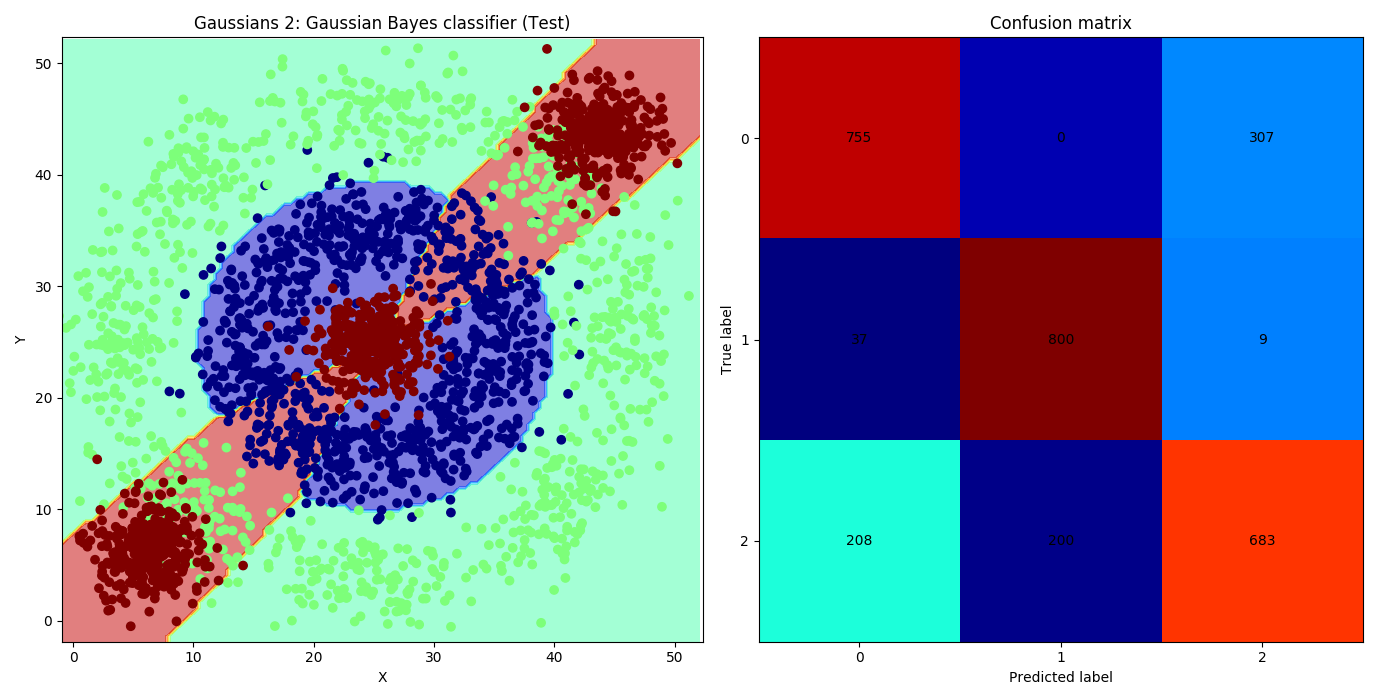
\includegraphics[width=0.8\linewidth]{figs/2-Bayes}
	\caption{Resultado del conjunto 2 con clasificador de Test Bayesiano}
	\label{fig:2-Bayes}
\end{figure}

\begin{figure}[!ht]
	\centering
	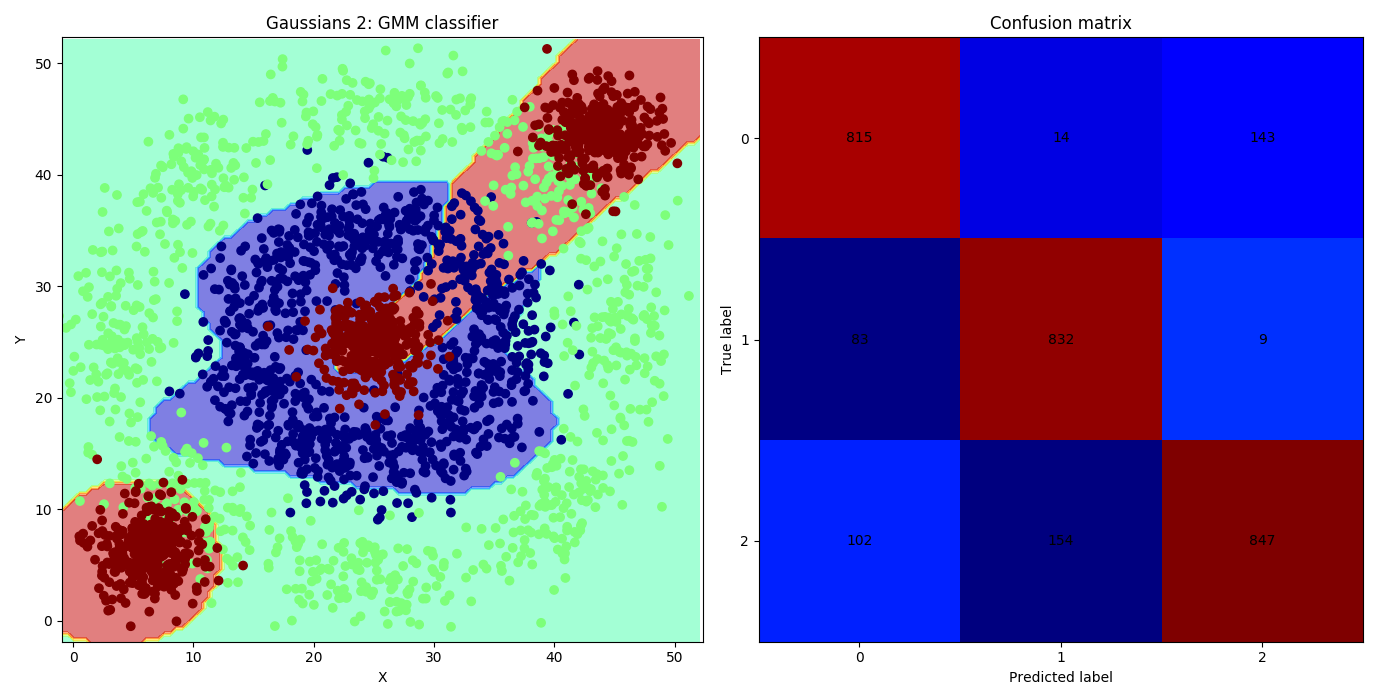
\includegraphics[width=0.8\linewidth]{figs/2-GMM}
	\caption{Resultado del conjunto 2 con clasificador de mezcla de gaussianas}
	\label{fig:2-GMM}
\end{figure}

\begin{figure}[!ht]
	\centering
	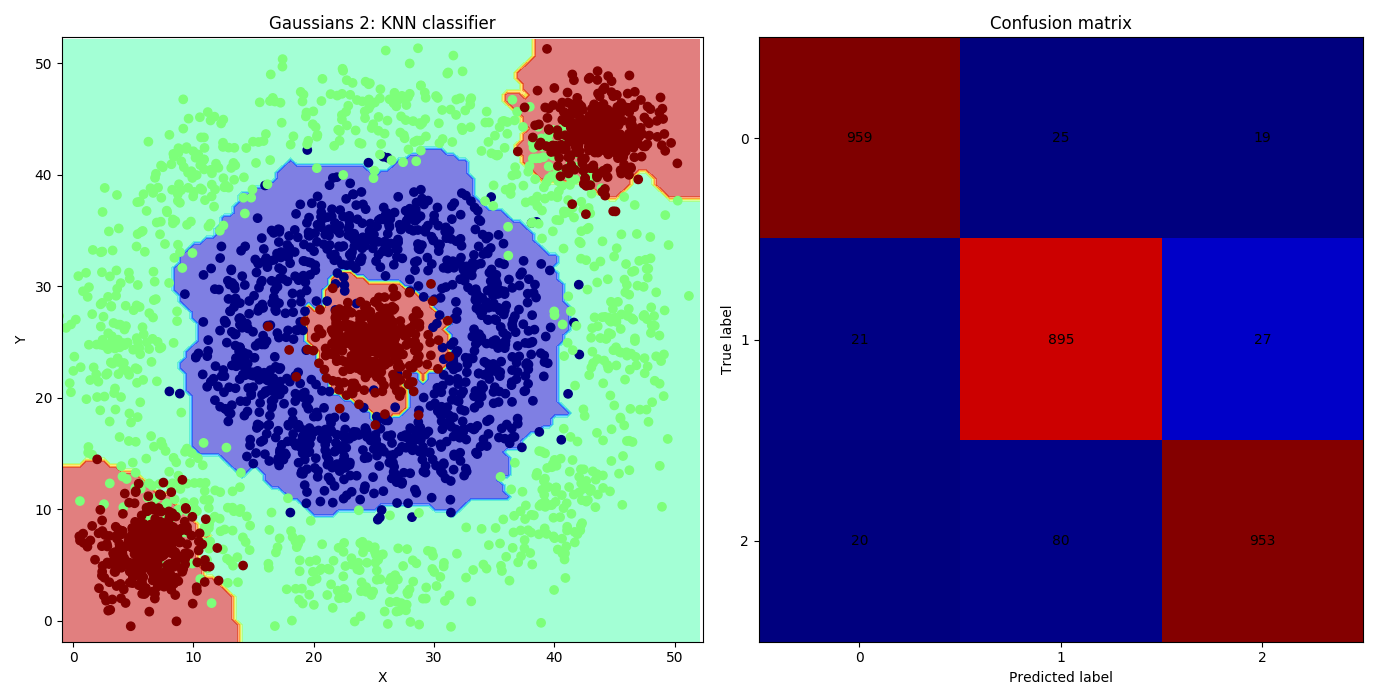
\includegraphics[width=0.8\linewidth]{figs/2-KNN}
	\caption{Resultado del conjunto 2 con clasificador de Vecinos mas cercanos (KNN)}
	\label{fig:2-KNN}
\end{figure}

\begin{figure}[!ht]
	\centering
	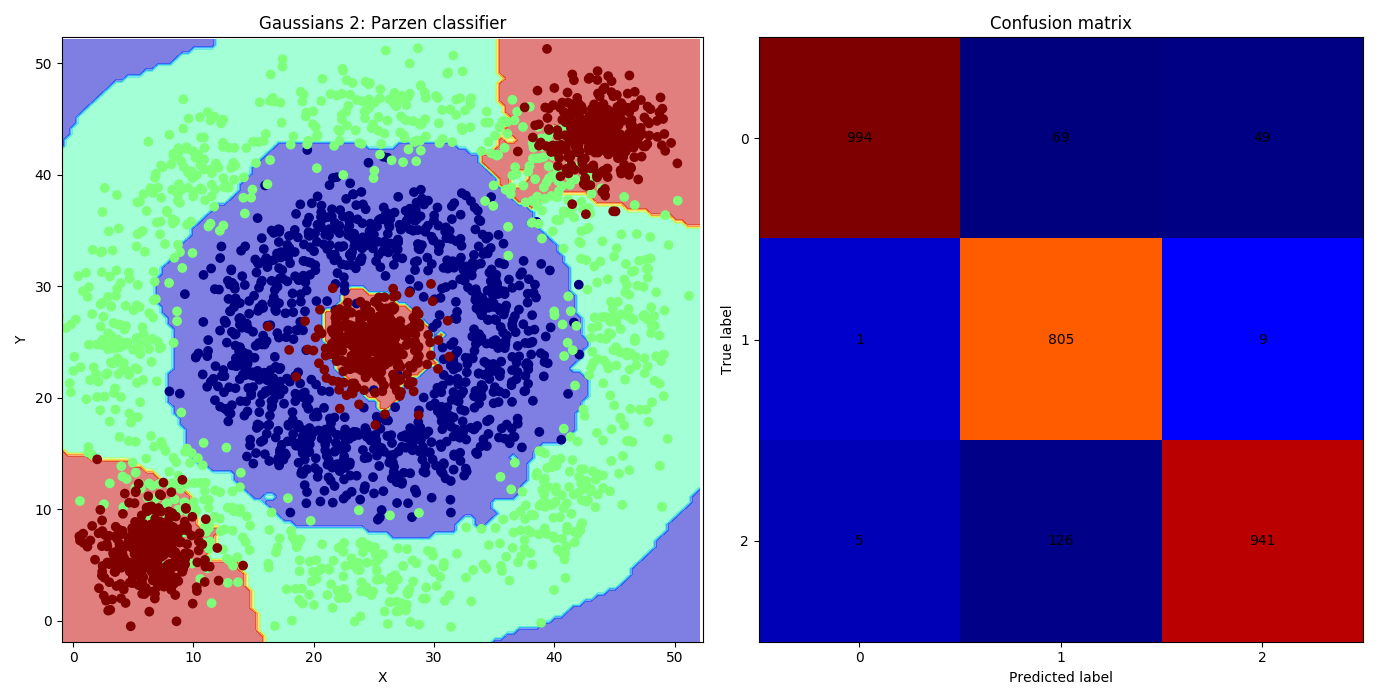
\includegraphics[width=0.8\linewidth]{figs/2-Parzen}
	\caption{Resultado del conjunto 2 con clasificador basado en ventanas de Parzen}
	\label{fig:2-Parzen}
\end{figure}

Para este conjunto de datos el clasificador que mejores resultados proporciona es el basado en los vecinos mas cercanos (KNN), el script seleccion� como par�metros �ptimos un K = 4 y pesos en funci�n de la distancia. A la vista de los resultados los modelos basados en gaussianas tienen problemas para adaptarse adaptarse a los datos, principalmente diferenciando entre las clases azul y verde.

\clearpage
\section{Resultados con Gaussianas 3}

\begin{figure}[!ht]
	\centering
	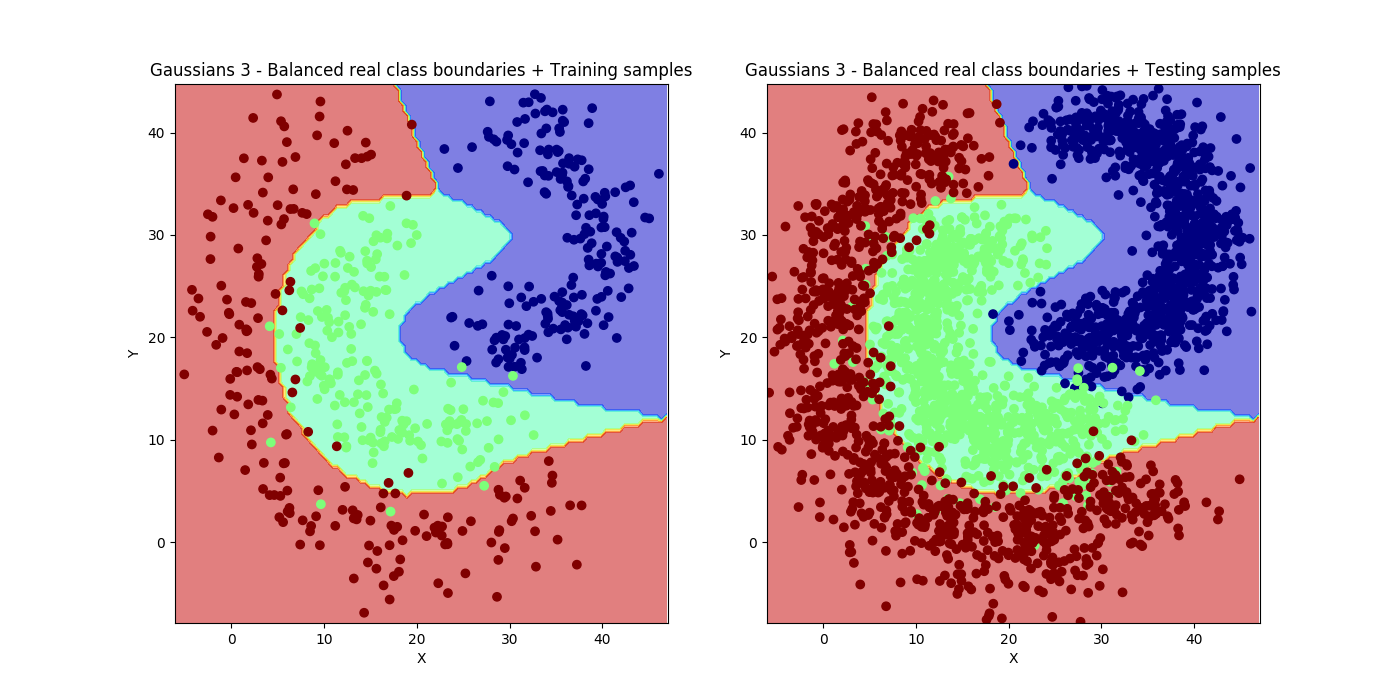
\includegraphics[width=0.8\linewidth]{figs/3-aTest}
	\caption{Conjunto de muestra 3}
	\label{fig:3-atest}
\end{figure}

El resultado obtenido para el conjunto de Gaussianas numero 3 es el siguiente:

\texttt{\small{
		Gaussian Bayes (Test) Done. Score: 0.93\\
		GMM Sk-Learn Done. Score: 0.94  n = [3, 2, 2] \\ Cov = ['tied', 'tied', 'spherical'] \\
		KNN Done. Score: 0.95  K = 3 Weights = uniform \\
		Parzen Done. Score: 0.94  r = 49 Weights = distance}}

\begin{figure}[!ht]
	\centering
	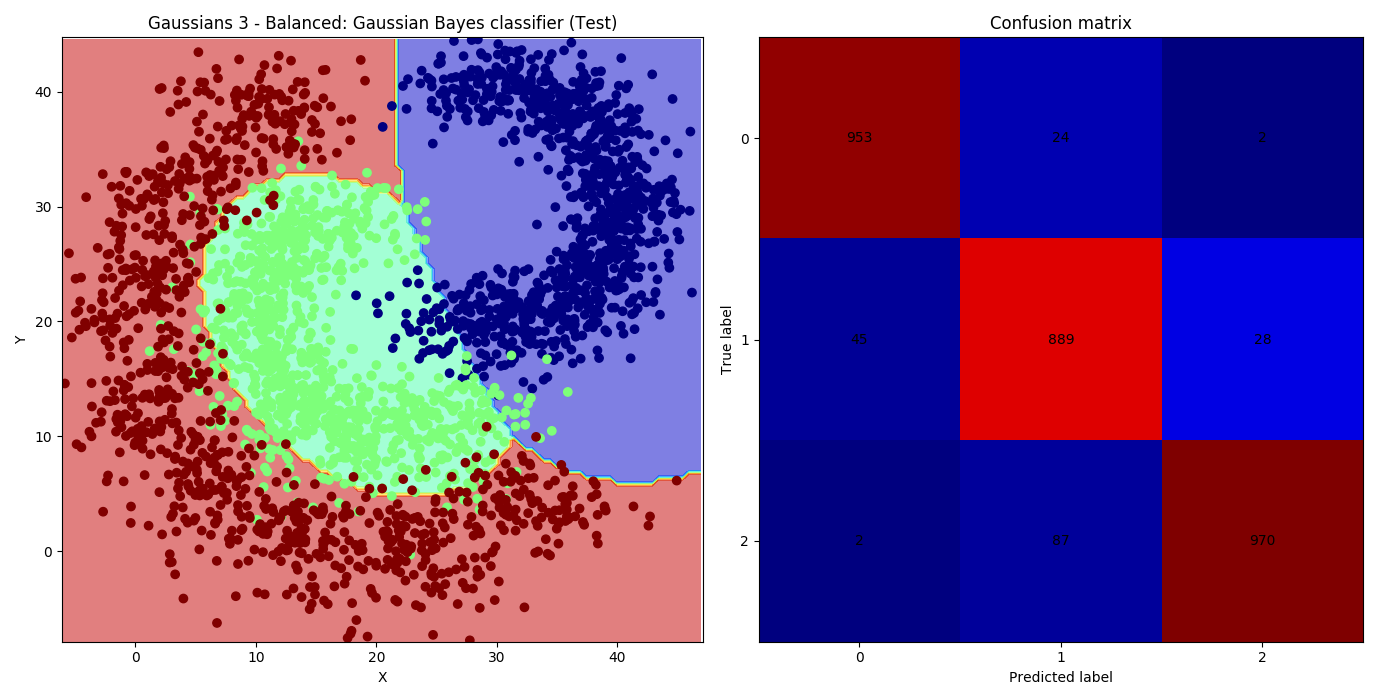
\includegraphics[width=0.8\linewidth]{figs/3-Bayes}
	\caption{Resultado del conjunto 3 con clasificador de Test Bayesiano}
	\label{fig:3-Bayes}
\end{figure}

\begin{figure}[!ht]
	\centering
	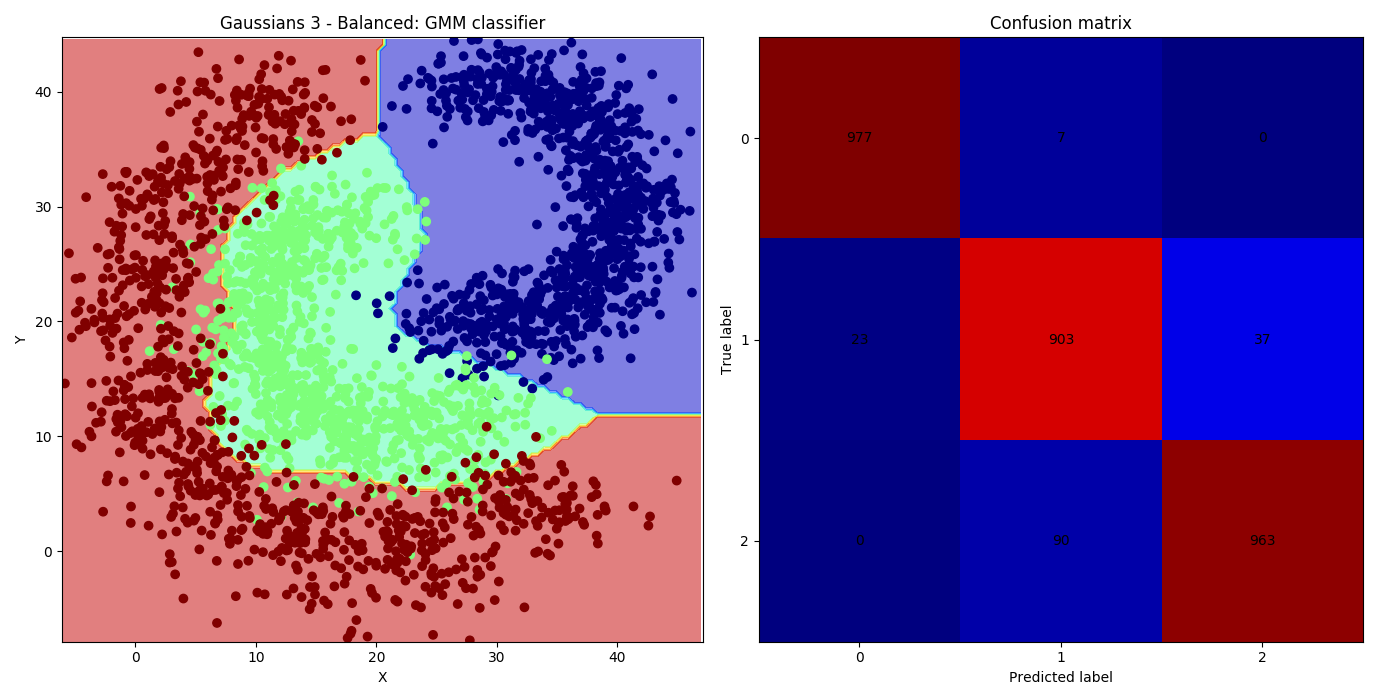
\includegraphics[width=0.8\linewidth]{figs/3-GMM}
	\caption{Resultado del conjunto 3 con clasificador de mezcla de gaussianas}
	\label{fig:3-GMM}
\end{figure}

\begin{figure}[!ht]
	\centering
	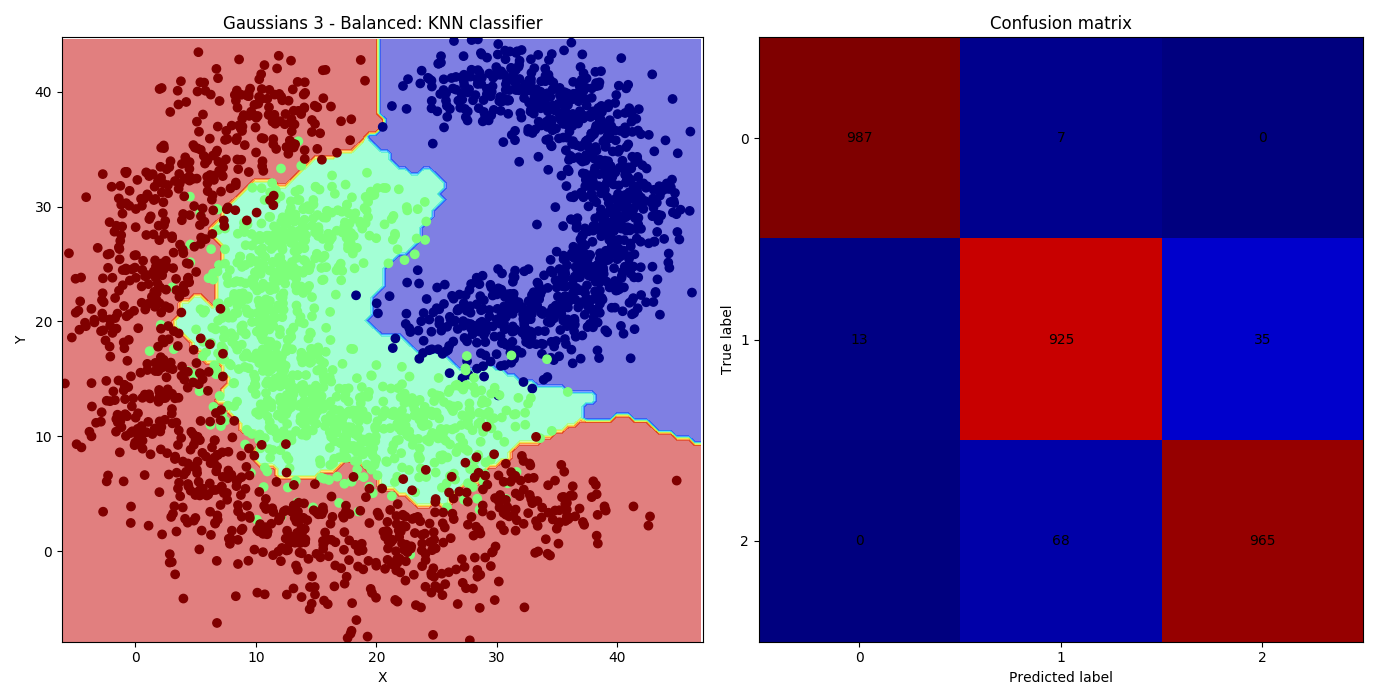
\includegraphics[width=0.8\linewidth]{figs/3-KNN}
	\caption{Resultado del conjunto 3 con clasificador de Vecinos mas cercanos (KNN)}
	\label{fig:3-KNN}
\end{figure}

\begin{figure}[!ht]
	\centering
	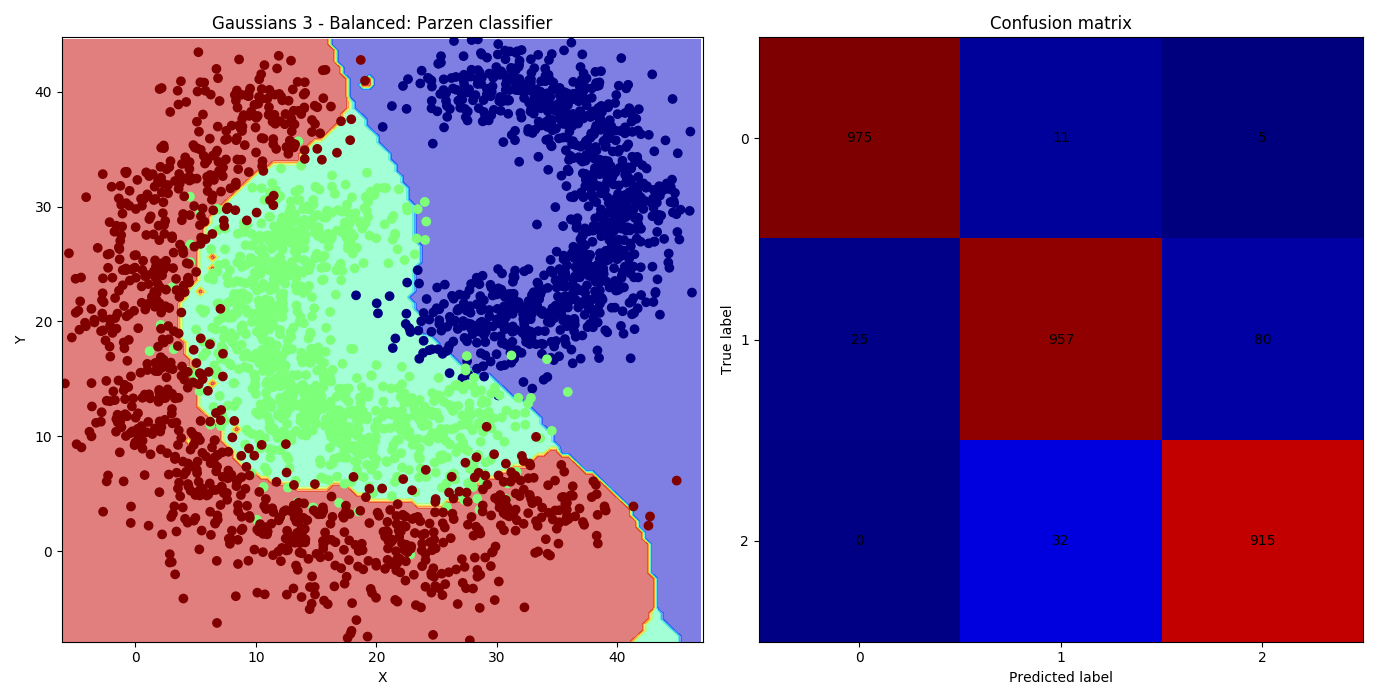
\includegraphics[width=0.8\linewidth]{figs/3-Parzen}
	\caption{Resultado del conjunto 3 con clasificador basado en ventanas de Parzen}
	\label{fig:3-Parzen}
\end{figure}

En este conjunto de entrenamiento el clasificador que mejores resultados presenta es KNN, debido principalmente a que los datos presentas datos muy pr�ximos y formas peculiares, a los que los modelos de gaussianas tienen problemas ajust�ndose

\clearpage
\section{Resultados con Gaussianas 4}

El resultado obtenido para el conjunto de Gaussianas numero 4 (desbalanceado) es el siguiente:

\texttt{\small{Gaussian Bayes (Test) Done. Score: 0.64 \\ 
		GMM Sk-Learn Done. Score: 0.96  n = [3, 3, 3] \\ Cov = ['spherical', 'diag', 'diag'] \\ 
		KNN Done. Score: 0.96  K = 12 Weights = uniform\\
		Parzen Done. Score: 0.64  r = 25 Weights = distance}}

\begin{figure}[!ht]
	\centering
	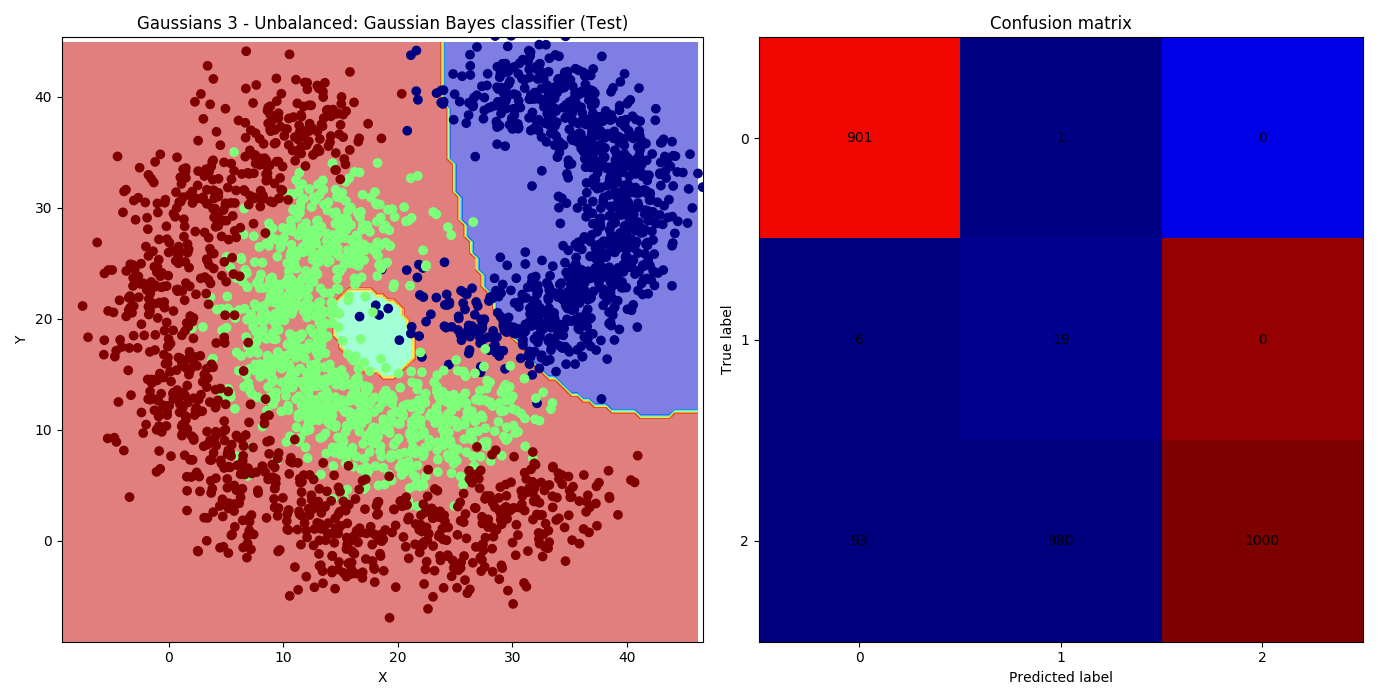
\includegraphics[width=0.8\linewidth]{figs/4-Bayes}
	\caption{Resultado del conjunto 4 (desbalanceado) con clasificador de Test Bayesiano}
	\label{fig:4-Bayes}
\end{figure}

\begin{figure}[!ht]
	\centering
	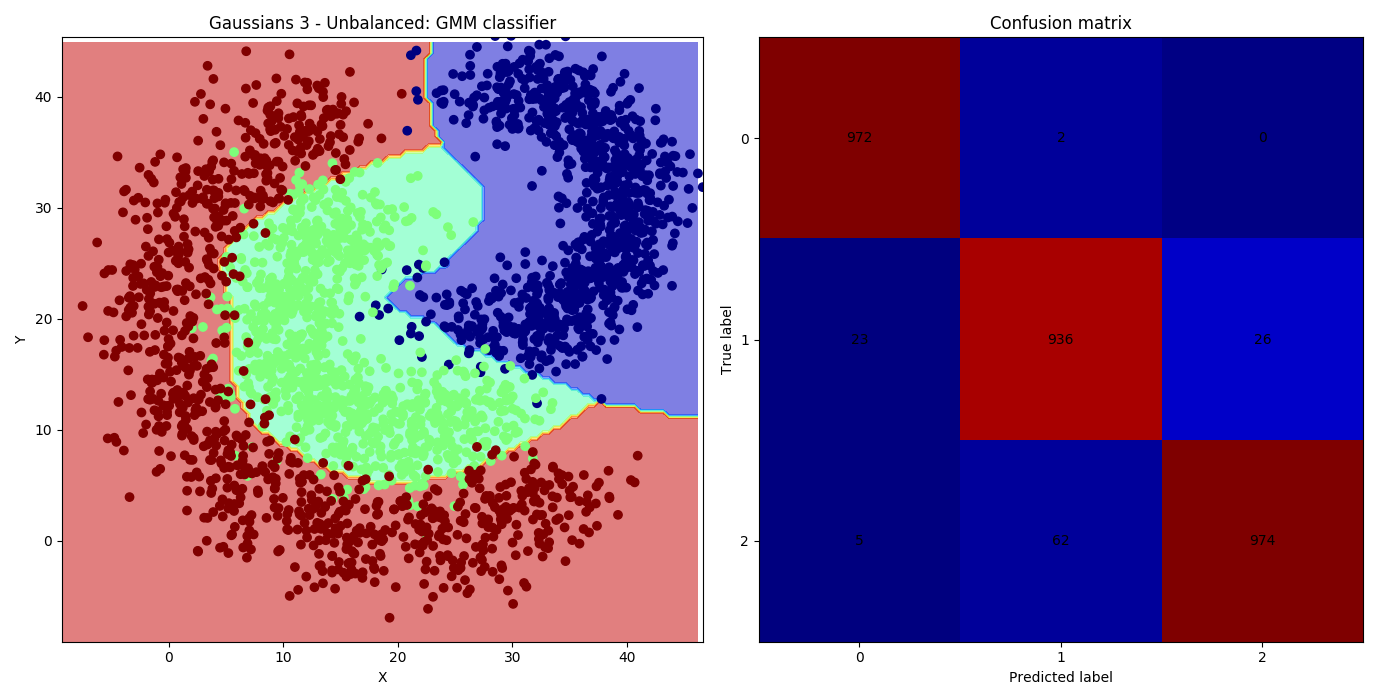
\includegraphics[width=0.8\linewidth]{figs/4-GMM}
	\caption{Resultado del conjunto 4 (desbalanceado) con clasificador de mezcla de gaussianas}
	\label{fig:4-GMM}
\end{figure}

\begin{figure}[!ht]
	\centering
	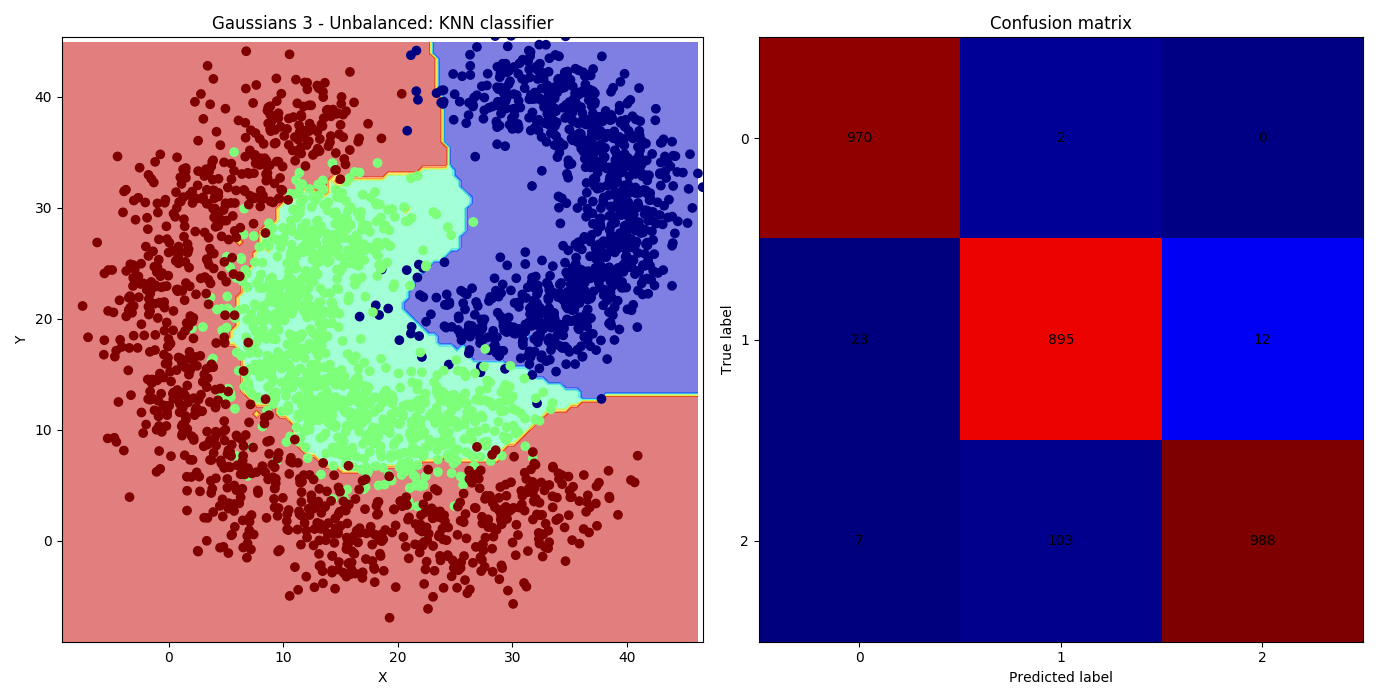
\includegraphics[width=0.8\linewidth]{figs/4-KNN}
	\caption{Resultado del conjunto 4 (desbalanceado) con clasificador de Vecinos mas cercanos (KNN)}
	\label{fig:4-KNN}
\end{figure}

\begin{figure}[!ht]
	\centering
	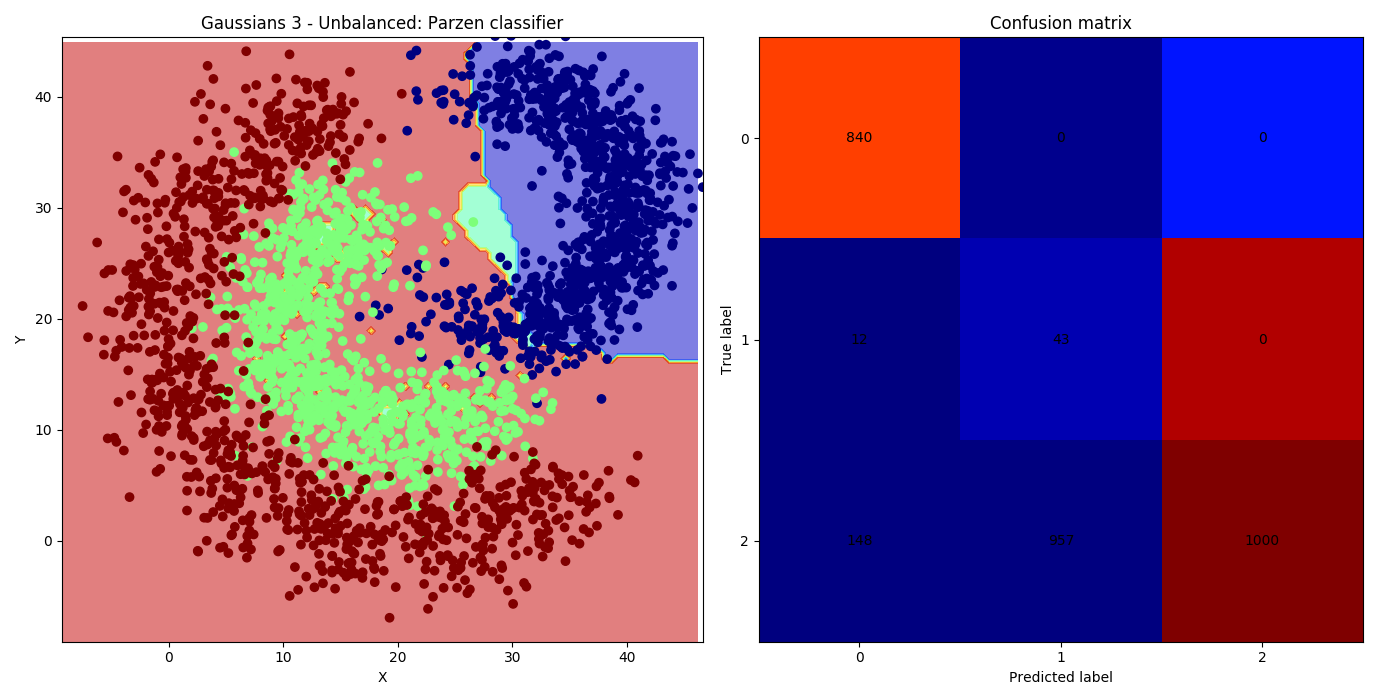
\includegraphics[width=0.8\linewidth]{figs/4-Parzen}
	\caption{Resultado del conjunto 4 (desbalanceado) con clasificador basado en ventanas de Parzen}
	\label{fig:4-Parzen}
\end{figure}

En este caso las clases presentan diferente numero de datos por clase, lo que repercute en el entrenamiento y el resultado de los clasificadores, para este conjunto el mejor se trata de nuevo de KNN,con un valor mayor de K que en casos anteriores. El basado en mezcla de gaussianas tambi�n tiene un buen  rendimiento y es capaz de realizar una buena estimaci�n de los datos con tan solo 3 gaussianas por clase.

\end{document}
